\chapter{Az \acrlong{off} projekt rövid áttekintése}

Az \acrlong{off} egy közösségi kezdeményezés, mely arra irányul, hogy minél több ember
tájékozhódhasson könnyen az élelmiszerek számos lényeges paraméteréről, így támogatva a
tudatos étkezést. Az alkalmazás segítségével több, mint másfélmillió élelmiszerről kaphatunk
információt. Az élelmiszerek elérhető fontosabb tulajdonságai a teljesség igénye nélkül:
\begin{itemize}
 \item Összetevők
 \item Allergén információk
 \item Tápérték adatok
 \item Nutri-score\footnote{Részletek a Nutri-score-ról: \url{https://hu.openfoodfacts.org/nutriscore}}
 \item Környezetre gyakorolt hatás
 \item Feldolgozottsági szint
\end{itemize}


Az alkalmazásban elérhető információk többségét a felhasználók maguk tölthetik fel az oldalra.
Ehhez használhatják például az \acrlong{off} applikációt az okostelefonjukon, melynek segítségével
beolvashatják egy adott termék vonalkódját, fotót készíthetnek róla, majd megadhatnak róla számtalan
részletet. A program támogatja az optikai szövegfelismerést (\acrfull{ocr}),
így akár a felhasználó időigényes közreműködése nélkül is ki tud nyerni lényeges információkat a
feltöltött képekből (\ref{fig:nutriextractionflow} ábra). Az így felvett információk bekerülnek egy adatbázisba, és így a program többi
felhasználója is szabadon hozzáférhet az adatokhoz.
\kep[0.045]{include/nutrifacts-extraction.png}{Az \acrlong{off} képes automatikusan is információkinyerésre a feltöltött képek alapján. Forrás: \cite{autodataextraction}}{nutriextractionflow}

Az \acrlong{off} natív Android és iOS applikáció mellett rendelkezik egy keresztplatformos,
Flutter-alapú alkalmazással is, továbbá egy webes alkalmazáson keresztül is hozzáférhetünk az
élelmiszerek adatához. Ezen kliensek kiszolgálásához a szoftvermérnökök egy klasszikus,
jól bevált megoldást választottak: a kliensek REST API segítségével kommunikálhatnak a % TODO: rest api szójegyzékbe
szerverrel. Az \acrlong{off} architektúrájának sematikus rajza \az{\ref{fig:offarchitektura}}
ábrán látható. A továbbiakban az architektúra szerver oldali részével nem foglalkozunk, az
ábrán kékkel jelölt mobilos kliensek közül is csak a natív Androidos alkalmazást nézzük meg részletesebben.

% tikz ábra beszúrása
\begin{figure}[h]
\centering
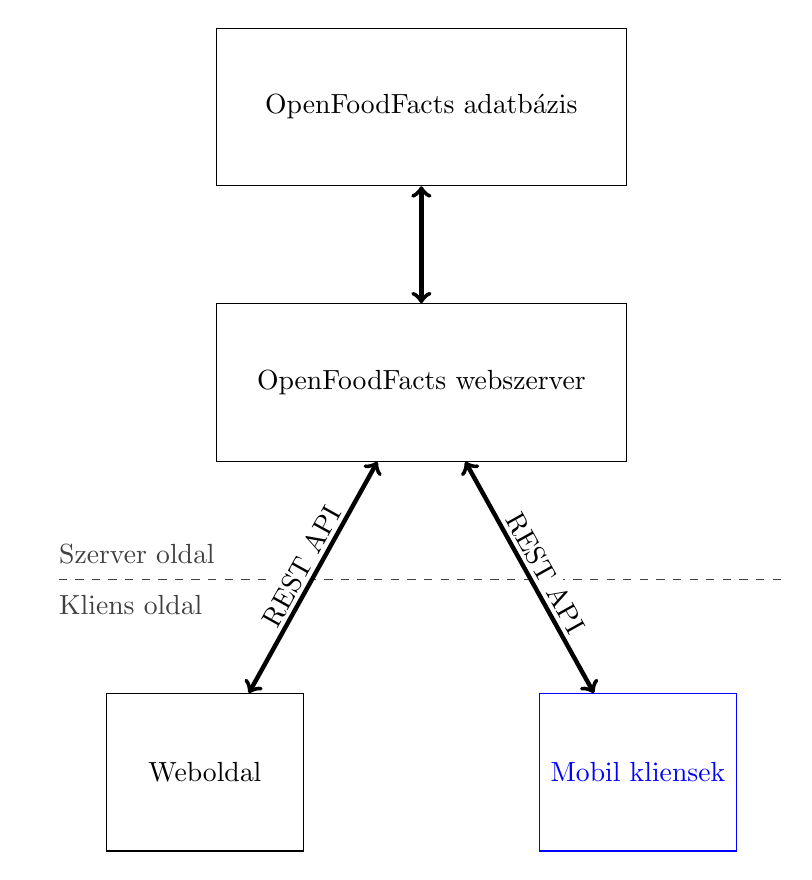
\begin{tikzpicture}[node distance=5cm and 1cm] \label{offarchitektura}
    \begin{scope}
        \node[shape=rectangle,draw,color=black, minimum height=2cm, minimum width=5.2cm] (OFFdb) { OpenFoodFacts adatbázis };
        \node[shape=rectangle, draw, color=black, minimum height=2cm, minimum width=5.2cm, yshift=1.5cm] (OFFwebsrv) [below of = OFFdb] { OpenFoodFacts webszerver };
            \begin{scope}[node distance=7cm]
                \node[shape=rectangle, draw, color=black, minimum height=2cm, minimum width=2.5cm, xshift=2.2cm] (OFFwebsite) [below left of = OFFwebsrv] { Weboldal };
                \node[shape=rectangle, draw, color=blue, minimum height=2cm, minimum width=2.5cm, xshift=-2.2cm] (mobileclients) [below right of = OFFwebsrv] { Mobil kliensek };
            \end{scope}
    \end{scope}
    \begin{scope}
        \path [clip] (-5,-8) rectangle (-1.88,-5) (-1.4,-8) rectangle (1.4,-5) (1.8,-8) rectangle (4.6,-5);
        \draw[darkgray, dashed] ([sloped, xshift=-2cm, yshift=-2.5cm]OFFwebsrv.west) to node [text width=3cm, anchor=west, above, xshift=-3.1cm, yshift=0.075cm] {Szerver oldal} node [text width=3cm, anchor=west, below, xshift=-3.1cm, yshift=-0.075cm] {Kliens oldal} ([sloped, pos=0.5, xshift=2cm, yshift=-2.5cm]OFFwebsrv.east);
    \end{scope}
    \draw[<->, ultra thick] (OFFdb) to node [sloped, pos=0.5, xshift=0.05cm, yshift=0.2cm] {} (OFFwebsrv);
    \draw[<->, ultra thick] (OFFwebsrv) to node [sloped, pos=0.5, xshift=0.05cm, yshift=0.2cm] {REST API} (OFFwebsite);
    \draw[<->, ultra thick] (OFFwebsrv) to node [sloped, pos=0.5, xshift=0.05cm, yshift=0.2cm] {REST API} (mobileclients);
\end{tikzpicture}

\caption{\centering Az \acrlong{off} rendszer architektúrája, a mobilos kliensek elhelyezkedése az architektúrában}
\label{fig:offarchitektura}
\end{figure}
